\documentclass{beamer}

\usepackage{amsmath,amssymb,amsthm}
\usepackage[all]{xy}
\usepackage{graphicx}



\numberwithin{equation}{subsection}

% Basic macros
\def\lim{\mathop{\mathrm{lim}}\nolimits}
\def\colim{\mathop{\mathrm{colim}}\nolimits}
\def\Spec{\mathop{\mathrm{Spec}}}
\def\Hom{\mathop{\mathrm{Hom}}\nolimits}
\def\Ext{\mathop{\mathrm{Ext}}\nolimits}
\def\Ker{\mathop{\mathrm{Ker}}}
\def\Im{\mathop{\mathrm{Im}}}
\def\Coker{\mathop{\mathrm{Coker}}}
 \def\Coim{\mathop{\mathrm{Coim}}}

% Slide numbering
\addtobeamertemplate{navigation symbols}{}{%
    \usebeamerfont{footline}%
    \usebeamercolor[fg]{footline}%
    \hspace{1em}%
    \insertframenumber/\inserttotalframenumber
}



\title{Deformations of Stanley-Reisner schemes}
\author{Daniel González Casanova Azuela}
\institute{PUC-Rio}
\date{Legalzinho\\ UFF\\[1em] December 4, 2025}

\begin{document}

\begin{frame}%Title page
\titlepage
\end{frame}


\section*{Objective}

\begin{frame}%Objective
\frametitle{Objective}
Show or disprove existence of a
Calabi-Yau threefold of degree 20 in $\mathbb{P}^7$
that degenerates to the Stanley-Reisner scheme of 
Grünbaum's triangulated 3-sphere with 8 vertices.
\end{frame}

\section*{Plan of the talk}
\label{section-plan}

\begin{frame}%Plan of the talk
\frametitle{Plan of the talk}
\tableofcontents
\end{frame}

\section{Stanley-Reisner schemes}
\begin{frame}%SR schemes
\frametitle{Stanley-Reisner schemes}
Let $[n]:=\{0,\ldots,n\}$, and let $\Delta_n$ denote the power set of $[n]$.

\medskip\noindent
A subset $\mathcal{K} \subseteq \Delta_n$ is called a {\it simplicial complex} 
if for every $f \in \mathcal{K}$ all the subsets of $f$ are
also in $\mathcal{K}$.
Elements of $\mathcal{K}$ are called {\it faces}.

\medskip\noindent
Let $S=\mathbb{C}[x_0,\ldots,x_n]$.
If $a=\{i_1,\ldots,i_k\}\in \Delta_n$ we write $x_a \in S$ 
for the square-free monomial $x_{i_1}\cdot\ldots\cdot x_{i_k}$.
The {\it Stanley-Reisner (SR)} ideal
of $\mathcal{K}$ is
{\bf generated by the monomials corresponding
to the ``non-faces''} of $\mathcal{K}$:
$$
I_{\mathcal{K}}=\left<x_p : p \in \Delta_n\setminus \mathcal{K}\right>
\subseteq S.
$$
The {\it SR ring} of $\mathcal{K}$ is
$A_{\mathcal{K}}=S/I_{\mathcal{K}}$
and the {\it SR scheme} is $\text{Proj} A_{\mathcal{K}}$.

\centering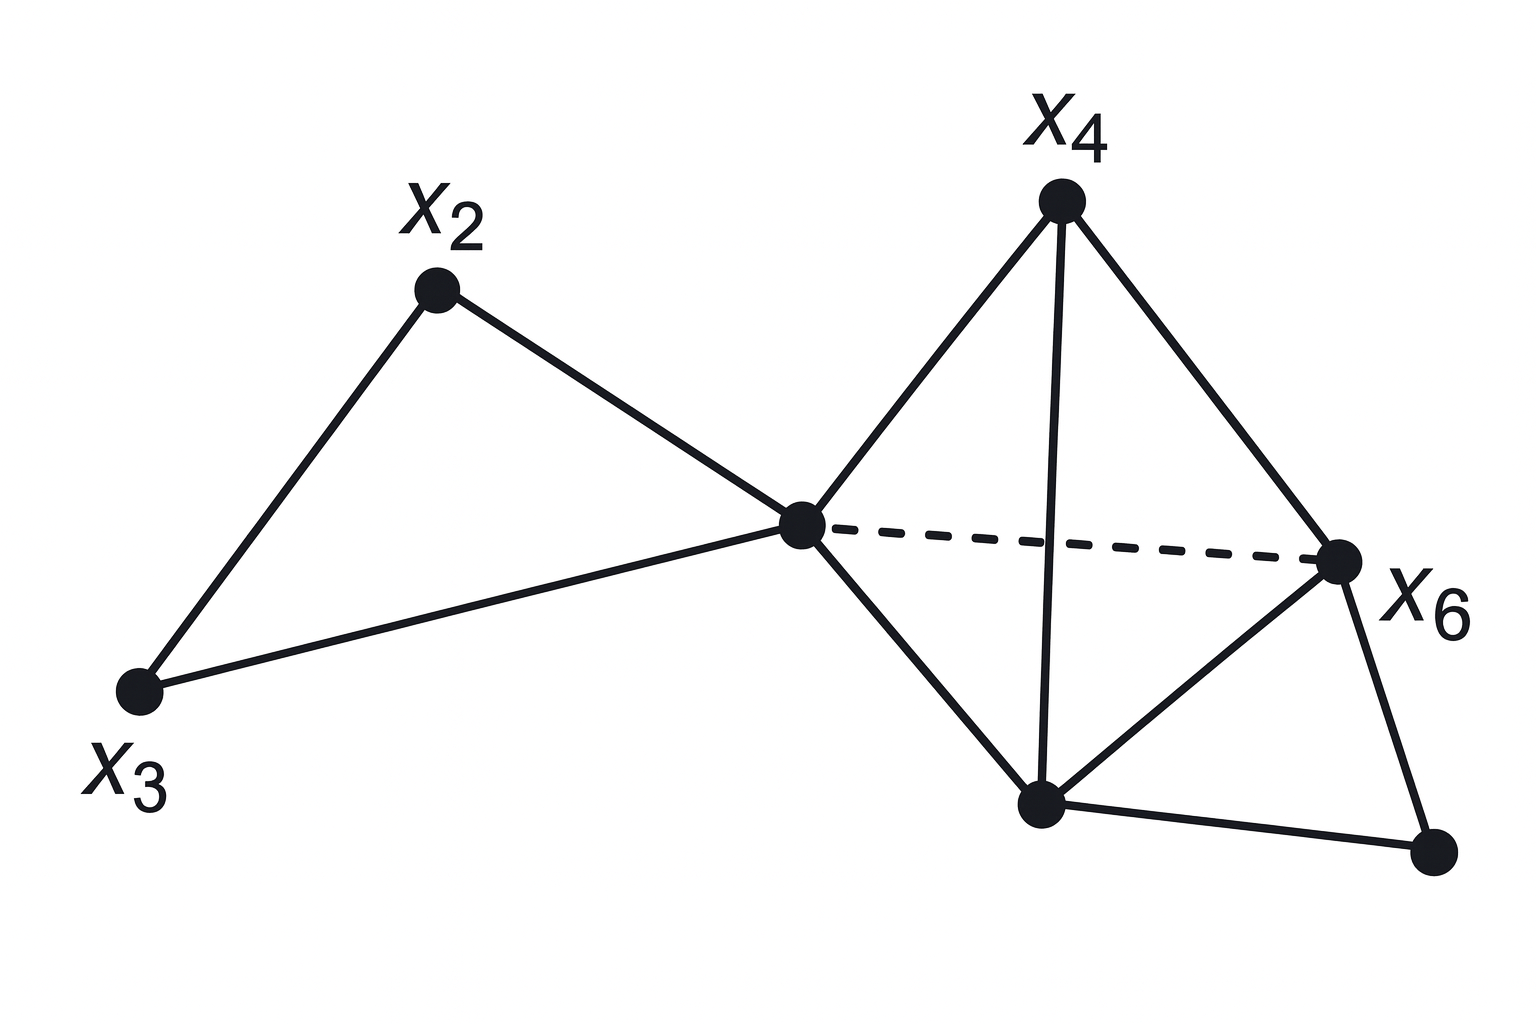
\includegraphics[width=.3\linewidth]{simplicial-complex.png}
\end{frame}

\section{Deformations}
\label{section-deformations}

\begin{frame}%Deformations
\frametitle{Deformations}
Let $X$ be scheme.
A {\it deformation} of $X$ is a Cartesian diagram 
$$
\xymatrix{
X\ar[r]\ar[d]&\mathcal{X}\ar[d]^{\pi}\\
\Spec \mathbb{C}\ar[r]&B
}
$$
where $\pi$ is a flat surjective morphism of algebraic $\mathbb{C}$-schemes and
$B$ is connected.

\medskip\noindent
A {\it smoothing} is a deformation where the general fibre $X_t$ 
of $\pi$ is smooth.
\end{frame}

\begin{frame}%Deformation of a hyperbola
\frametitle{Example: deformation of a hyperbola}
Consider the deformation
$$
\xymatrix{
\Spec\frac{\mathbb{C}[x,y]}{(xy-1)}\ar[r]\ar[d]
&\Spec\frac{\mathbb{C}[x,y,t]}{(xy-t)}\ar[d]\\
\Spec\frac{\mathbb{C}[t]}{(t-1)}\ar[r]
&\Spec \mathbb{C}[t]
}
$$
where $\pi:\mathcal{X} \to B$ be the morphism
determined by the natural homomorphism
$\mathbb{C}[t] \to \mathbb{C}[x,y,t]/(ty-x^2)$.

\medskip\noindent
The generic fibre is a (smooth) hyperbola 
while the fibre at $t=0$ is singular and reducible.
\end{frame}

\begin{frame}%Example: smoothing of a SR scheme
\frametitle{Example: smoothing of a SR scheme}

Consider the
simplicial complex $\bullet-\bullet-\bullet-\bullet$.
It's SR ideal is generated by
$$
x_0x_2,\qquad x_0x_3,\qquad x_1x_3.
$$
The twisted cubic is a smoothing of this variety.
Recall that the {\it twisted cubic} is the image 
of the Veronesse map of degree 3,
\begin{align*}
\nu: \mathbb{P}^1 &\longrightarrow \mathbb{P}^3 \\
[u:v] &\longmapsto [u^3:u^2v:uv^2:v^3]=[x_0:x_1:x_2:x_3],
\end{align*}
and its ideal is generated by
$$
x_1^2-x_0x_2,\quad x_1x_2-x_0x_3,\quad x_2^2-x_1x_3.
$$
\end{frame}

\begin{frame}%Example: smoothing of a SR scheme
\frametitle{Example: smoothing of a SR scheme}
To construct a deformation between these two schemes
we introduce a new variable:
$$
x_0\rightsquigarrow t^ax_0,\qquad 
x_1\rightsquigarrow t^bx_1,\qquad 
x_2\rightsquigarrow t^cx_2,\qquad 
x_3\rightsquigarrow t^dx_3.
$$
The equations of the twisted cubic become
$$
\xymatrix{
x_1^2-x_0x_2,\ar@{~>}[d]
&x_1x_2-x_0x_3,\ar@{~>}[d]
&x_2^2-x_1x_3\ar@{~>}[d]\\
t^{2b}x_1^2-t^{a+c}x_0x_2,
&t^{b+c}x_1x_2-t^{a+d}x_0x_3,
&t^{2c}x_2^2-t^{b+d}x_1x_3.
}
$$
\pause
To arrive at the equations of the SR scheme as $t \to 0$
we need
\begin{align*}
2b>a+c,\qquad b+c>a+d,\qquad 2c>b+d.
\end{align*}
A solution is $a=1,b=2,c=2,d=0$.
\end{frame}

\section{Gröbner degenerations}

\begin{frame}%Gröbner degenerations
\frametitle{Gröbner degenerations}
Let $k$ be any field and $k[x_1,\ldots,x_n]$. 
Denote the monomials in 
$k[x_1,\ldots,x_n]$ by $\mathbf{x}^a=x_1^{a_1}\ldots x_n^{a_n}$,
where $\mathbf{a}=(a_1,\ldots,a_n)\in \mathbb{N}^n$.
Fix a weight vector $\omega=(\omega_1,\ldots,\omega_n)\in\mathbb{R}^n$.

\medskip\noindent
For any
polynomial $f=\sum c_i \mathbf{x}^{\mathbf{a}_i}$ we define the 
{\it initial form} $\text{in}_\omega(f)$ to be the sum of all terms
$c_i\mathbf{x}^{\mathbf{a}_i}$ such that the inner product $\omega\mathbf{a}_i$
is maximal. 

\medskip\noindent
For an ideal $I$ we define the {\it initial ideal} to be the ideal
generated by all initial forms:
$$
\text{in}_\omega(I):=\langle\text{in}_\omega(f):f\in I\rangle.
$$
\end{frame}

\begin{frame}%Gröbner degenerations
\frametitle{Gröbner degenerations}
Let's apply this to our example of the twisted cubic.
\[
\begin{array}{cccc}
\textbf{SR}(\bullet-\bullet-\bullet-\bullet) & x_0x_2, & x_0x_3, & x_1x_3 \\
\textbf{twisted cubic} 
& x_1^2-x_0x_2, & x_1x_2-x_0x_3, & x_2^2-x_1x_3.
\end{array}
\]
Consider the weight vector $\omega=(5,-5,-5,5)$.
The inner products of $\omega$ with the vectors $\mathbf{a}_i$
in the generators of the ideal for the twisted cubic are
\begin{align*}
\omega\cdot(0,2,0,0)&=-10,\qquad \omega\cdot(1,0,1,0)=0\\
\omega\cdot(0,1,1,0)&=-10,\qquad \omega\cdot(1,0,0,1)=10\\
\omega\cdot(0,0,2,0)&=-5,\qquad \omega\cdot(0,1,0,1)=0
\end{align*}

\noindent
The initial ideal is the ideal of the SR scheme.
\end{frame}

\begin{frame}%Gröbner degenerations
\frametitle{Gröbner degenerations}

\begin{theorem}[Eisenbud, Commutative Algebra with a view…]
\label{theorem-grobner-flat-morphism}
For any ideal $I \subset k[x_1,\ldots,x_r]:=S$, the
$k[t]$-algebra $S[t]/\tilde{I}$ is free ---and thus flat---
as a $k[t]$ module. Furthermore,
$$
S[t]/\tilde{I}\otimes_{k[t]}k[t,t^{-1}]
\cong S[t]/I[t,t^{-1}],
$$
while
$$
S[t]/\tilde{I}\otimes_{k[t]}k[t]/(t)
\cong S[t]/\text{in}_{\omega}(I).
$$

Thus $S[t]/\tilde{I}$ is a flat family over $k[t]$ of quotients
of $S$ whose fiber over $0$ is $S/\text{in}_\omega(I)$ and
whose fiber over any $(t-u)$ for $0 \neq u \in k$ is $S/I$.
\end{theorem}


\end{frame}

\section{Grünbaum sphere}

\begin{frame}%Grünbaum sphere
\frametitle{Grünbaum sphere}

{\footnotesize
\begin{thebibliography}{1}
\bibitem{grun}
B. Grünbaum and V.~P. Sreedharan,
\emph{An enumeration of simplicial 4-polytopes with 8 vertices},
J. Combin. Theory, 2 (1967), 437–465.
\end{thebibliography}
}

\medskip\noindent
Grünbaum-Shreedharan discovered a simplicial complex $\mathcal{M}$ 
which is not the boundary of a 4-polytope
despite being a triangulation of the 3-sphere.

\pause\medskip\noindent
A smoothing of $\text{SR}(\mathcal{M})$ would
be a CY 3-fold of degree 20 in $\mathbb{P}^7$:
\begin{lemma}
\label{lemma-degree}
The number of maximal facets of a triangulation equals the
degree of the associated variety.
\end{lemma}

\begin{theorem}
\label{theorem-smoothing-triangulation}
If it exists, a smoothing of the SR scheme of a 
triangulation of the 3-sphere yields a Calabi-Yau threefold.
\end{theorem}

\noindent
\end{frame}

\begin{frame}%A smooth candidate
\frametitle{A smooth candidate}

There exists a CY threefold in $\mathbb{P}^7$ of degree
20 that was first studied 
by Gulliksen-Neg\aa ard.
Its ideal is generated by the
$3\times 3$ minors of $4\times 4$ matrix with linear forms.

\medskip\noindent
For example,
$$
\begin{bmatrix}
x_1 & x_2 & x_3 & x_4 \\
x_5 & x_6 & x_7 & x_8 \\
x_2 & x_3 & x_4 & x_5 \\
x_6 & x_7 & x_8 & x_1
\end{bmatrix}
$$
\end{frame}

\begin{frame}%
\frametitle{A perfect matching?}
\vspace{-1em}{\tiny
\begin{align*}
\text{SR}(\mathcal{M})\qquad \qquad & 
\qquad \qquad \qquad \qquad \qquad \quad \text{GN}\\ 
x_6x_7x_8,\qquad \qquad 
&x_3^2 x_5 - x_2 x_4 x_5 - x_2 x_3 x_6 + x_1 x_4 x_6 + x_2^2 x_7 - x_1 x_3 x_7, \\
x_4x_6x_8,\qquad \qquad &-x_3 x_6^2 + x_3 x_5 x_7 + x_2 x_6 x_7 - x_1 x_7^2 - x_2 x_5 x_8 + x_1 x_6 x_8, \\
x_3x_7x_8,\qquad \qquad &-x_3^2 x_6 + x_2 x_4 x_6 + x_2 x_3 x_7 - x_1 x_4 x_7 - x_2^2 x_8 + x_1 x_3 x_8, \\
x_3x_5x_7,\qquad \qquad &x_4 x_6^2 - x_4 x_5 x_7 - x_3 x_6 x_7 + x_2 x_7^2 + x_3 x_5 x_8 - x_2 x_6 x_8, \\
x_3x_4x_8,\qquad \qquad &x_3 x_4 x_5 - x_2 x_5^2 - x_2 x_4 x_6 + x_1 x_5 x_6 + x_2^2 x_8 - x_1 x_3 x_8, \\
x_2x_7x_8,\qquad \qquad 
&-x_1 x_2 x_5 + x_1^2 x_6 - x_4 x_6^2 + x_4 x_5 x_7 + x_2 x_6 x_8 - x_1 x_7 x_8, \\
x_2x_5x_7,\qquad \qquad 
&-x_1 x_2^2 + x_1^2 x_3 - x_3 x_4 x_6 + x_2 x_5 x_6 + x_2 x_4 x_7 - x_1 x_5 x_7, \\
x_2x_5x_6,\qquad \qquad 
&x_1 x_3 x_5 - x_1 x_2 x_6 + x_5 x_6^2 - x_5^2 x_7 - x_3 x_6 x_8 + x_2 x_7 x_8, \\
x_2x_4x_7,\qquad \qquad 
&x_4^2 x_5 - x_3 x_5^2 - x_2 x_4 x_7 + x_1 x_5 x_7 + x_2 x_3 x_8 - x_1 x_4 x_8, \\
x_2x_4x_6,\qquad \qquad 
&-x_1 x_3 x_5 + x_1^2 x_7 - x_4 x_6 x_7 + x_4 x_5 x_8 + x_3 x_6 x_8 - x_1 x_8^2, \\
x_1x_4x_6,\qquad \qquad 
&-x_1 x_2 x_3 + x_1^2 x_4 - x_4^2 x_6 + x_3 x_5 x_6 + x_2 x_4 x_8 - x_1 x_5 x_8, \\
x_1x_4x_5,\qquad \qquad 
&x_1 x_4 x_5 - x_1 x_2 x_7 + x_5 x_6 x_7 - x_5^2 x_8 - x_4 x_6 x_8 + x_2 x_8^2, \\
x_1x_3x_8,\qquad \qquad 
&x_4^2 x_6 - x_3 x_5 x_6 - x_3 x_4 x_7 + x_2 x_5 x_7 + x_3^2 x_8 - x_2 x_4 x_8, \\
x_1x_3x_6,\qquad \qquad 
&-x_1 x_3 x_6 + x_1 x_2 x_7 - x_4 x_7^2 + x_4 x_6 x_8 + x_3 x_7 x_8 - x_2 x_8^2, \\
x_1x_3x_5,\qquad \qquad 
&-x_1 x_3^2 + x_1 x_2 x_4 - x_4^2 x_7 + x_3 x_5 x_7 + x_3 x_4 x_8 - x_2 x_5 x_8, \\
x_1x_2x_5,\qquad \qquad 
&x_1 x_4 x_6 - x_1 x_3 x_7 + x_5 x_7^2 - x_5 x_6 x_8 - x_4 x_7 x_8 + x_3 x_8^2
\end{align*}}
\end{frame}

\iffalse %Whoa! It looks like there was a mistake in this!
%The minimal resolutions actually are the same!!
\begin{frame}%Minimal resolutions
\frametitle{Minimal resolutions}

\begin{align*}
\textbf{twisted cubic}\qquad &
\xymatrix@C=1em{
0\ar[r]&\mathcal{O}(-3)^{\oplus 2}\ar[r]^{d_2}&
\mathcal{O}(-2)^{\oplus 3}\ar[r]^-{d_1}&
\mathcal{O}_{\mathbb{P}^3}\ar[r]&\mathcal{O}_X\ar[r]&0
}\\
\textbf{SR}(\bullet-\bullet-\bullet-\bullet)\qquad&
\xymatrix@C=1em{
0\ar[r]&\mathcal{O}(-3)^{\oplus 2}\ar[r]^{d_2}&
\mathcal{O}(-2)^{\oplus 3}\ar[r]^-{d_1}&
\mathcal{O}_{\mathbb{P}^3}\ar[r]&\mathcal{O}_X\ar[r]&0
}
\end{align*}
\vspace{-1em}
\pause\begin{align*}
\xymatrix@C=.9em@R=.2em{\textbf{GN}
&
0 \ar[r] &
\mathcal{O}(-4) \ar[r] &
\mathcal{O}(-3)^{\oplus 16} \ar[r] &
\mathcal{O}(-2)^{\oplus 30} \ar[r] &
\mathcal{O}(-1)^{\oplus 16} \ar[r] &
\mathcal{O}
\\
\textbf{SR}(\mathcal{M})&
0 \ar[r] &
F_4 \ar[r] &
F_3 \ar[r] &
F_2 \ar[r] &
F_1 \ar[r] &
\mathcal{O}
}
\end{align*}
\vspace{-1em}
\begin{align*}
F_1 &= \mathcal{O}(-1)^{\oplus 5}\;\oplus\;\mathcal{O}(-2)^{\oplus 2}\;\oplus\;\mathcal{O}(-3)^{\oplus 4},\\
F_2 &= \mathcal{O}(-1)^{\oplus 6}\;\oplus\;\mathcal{O}(-2)^{\oplus 5}\;\oplus\;\mathcal{O}(-3)^{\oplus 12},\\
F_3 &= \mathcal{O}(-1)^{\oplus 2}\;\oplus\;\mathcal{O}(-2)^{\oplus 4}\;\oplus\;\mathcal{O}(-3)^{\oplus 12},\\
F_4 &= \mathcal{O}(-2)\;\oplus\;\mathcal{O}(-3)^{\oplus 4}.
\end{align*}

\end{frame}
\begin{frame}
\frametitle{Betti numbers and deformations}

\begin{minipage}{0.45\textwidth}
\centering
\textbf{GN}
\vspace{1em}

\begin{tabular}{c|ccccc}
 & 0 & 1 & 2 & 3 & 4 \\
\hline
total & 1 & 16 & 30 & 16 & 1 \\
0 & 1 & . & . & . & . \\
1 & . & . & . & . & . \\
2 & . & 16 & 30 & 16 & . \\
3 & . & . & . & . & . \\
4 & . & . & . & . & 1 \\
\end{tabular}
\end{minipage}
\hfill
\begin{minipage}{0.45\textwidth}
\centering
\textbf{SR}$(\mathcal{M})$
\vspace{1.5em}

\begin{tabular}{c|ccccc}
 & 0 & 1 & 2 & 3 & 4 \\
\hline
total & 1 & 11 & 23 & 18 & 5 \\
0 & 1 & . & . & . & . \\
1 & . & 5 & 6 & 2 & . \\
2 & . & 2 & 5 & 4 & 1 \\
3 & . & 4 & 12 & 12 & 4 \\
\end{tabular}
\end{minipage}

\vspace{1em}
It is a well-known fact of Gröbner degenerations that
$$
\beta_{ij}(S/I)\leq \beta_{ij}(S/\text{in}(I)).
$$
where $F_i=\bigoplus_jS(-j)^{\beta_{ij}}$.
{\footnotesize
\begin{thebibliography}{1}
\bibitem{conca2020}
A. Conca and M. Varbaro,
\emph{Square-free Groebner degenerations},
arXiv:1805.11923 [math.AC], 2020.
\end{thebibliography}
}
\end{frame}
\fi

\section{Big picture}

\begin{frame}%A triangulation of CP2
\frametitle{A triangulation of $\mathbb{C}P^2$}

{\footnotesize
\begin{thebibliography}{1}
\bibitem{KuhnelBanchoff1983}
W. K{\"u}hnel and T. F. Banchoff,
\emph{The 9-vertex complex projective plane},
The Mathematical Intelligencer, 5(3) (1983), 11--22.
\end{thebibliography}
}

\medskip\noindent
Künhel-Banchoff
discovered a triangulation of $\mathbb{C}P^2$ 
with 9 vertices
whose link is $\mathcal{M}$.

\medskip\noindent
For a face $f \in \mathcal{K}$,
the {\it link} of $f$ is the set
$$
\text{lk}(f,K)=\{g \in \mathcal{K}
:g\cap f=\emptyset, g \cup  f\in \mathcal{K}\}.
$$
\centering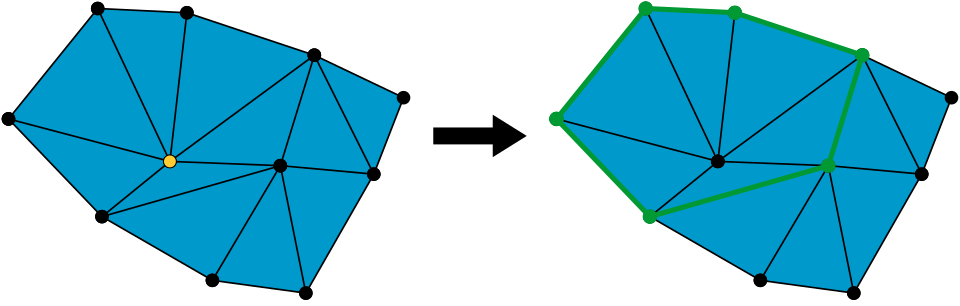
\includegraphics[width=0.7\textwidth]{link.png}
\end{frame}

\begin{frame}%Degenerations of generalised Kummer type fourfolds
\frametitle{Degenerations of generalised Kummer type fourfolds}

From a 2024 talk by Calla Tschanz presented in 
conference Kummers in Kraków:

\vspace{2em}
\begin{quotation}
``Aim: construct a type III
degeneration of varieties of generalised Kummer type 4-folds
with polarisation degree 2,
by starting from a given special fibre and constructing a smoothing.

Corollary. Proving this result will imply that a 
general HK variety of this type with polarisation
degree 2 (\& fixed divisibility) is contained
in 36 quartics.
(In particular, it is not contained in a cubic.)''
\end{quotation}
\end{frame}

\begin{frame}%References
\frametitle{References}

{\scriptsize
\begin{thebibliography}{1}
\bibitem{Eisenbud}
D. Eisenbud,
\emph{Commutative Algebra: With a View Toward Algebraic Geometry},
Springer, 1995.

\bibitem{Eisenbud-syzygies}
D. Eisenbud,
\emph{The Geometry of Syzygies: A Second Course in Commutative Algebra and 
Algebraic Geometry},
Springer, 2004.

\bibitem{BAYER19911}
D. Bayer and D. Eisenbud,
\emph{Graph curves},
Advances in Mathematics, 86(1) (1991), 1--40.

\bibitem{Fausk}
I. Fausk,
\emph{Pfaffian Calabi-Yau threefolds, Stanley-Reisner schemes and mirror symmetry},
PhD thesis, 2012.

\bibitem{grun}
B. Grünbaum and V.~P. Sreedharan,
\emph{An enumeration of simplicial 4-polytopes with 8 vertices},
J. Combin. Theory, 2 (1967), 437–465.

\bibitem{conca2020}
A. Conca and M. Varbaro,
\emph{Square-free Groebner degenerations},
arXiv:1805.11923 [math.AC], 2020.

\bibitem{KuhnelBanchoff1983}
W. K{\"u}hnel and T. F. Banchoff,
\emph{The 9-vertex complex projective plane},
The Mathematical Intelligencer, 5(3) (1983), 11--22.

\bibitem{callatalk}
C. Tschanz,
\emph{Talk at Kummers in Kraków (2024)},
\url{https://www.callatschanz.com/talks-and-travels}.
\end{thebibliography}
}

\end{frame}

\begin{frame}%Thank you
\centering
\LARGE Thank you!
\end{frame}

\bibliography{my}
\bibliographystyle{amsalpha}

\end{document}
